%\section{Modified Model with Length Control}
\section{Methodology}
\label{sec:approach}
%\section{Basic CNN Seq2seq Model}
%\label{sec:model}

In this section, we will describe the model architecture used for our experiments
and propose our length control method which is implemented by extending the 
basic model.
%Besides, we use existing length control method to control the
%summaries length of other methods for comparison and make sure that the length of summaries are less
%than 100 ~\footnote{The maximum length of summaries in CNN/DailyMail dataset is 94.}.
%This method doesn't change the model.

For summarization problems based on seq2seq model, 
given a sequence of tokens $\textbf{x} = (x_{1},x_{2},...,x_{m})$ in the
source document and a sequence of tokens
$\textbf{y} = (y_{1}, y_{2},..., y_{n})$ in the target summary (i.e. $m>n$),
the goal is to estimate the conditional probability
$p(\textbf{y}|\textbf{x})$:
\begin{equation}
p(\textbf{y} | \textbf{x}) \!=\! {\prod^T_{t} {p(y_{t} | y_{1}, y_{2},..., y_{t-1}, \textbf{x}})}
\end{equation}

We aim at getting the above conditional probabaility which can generate
summaries with arbitrary desired length.

\subsection{Basic CNN seq2seq Model}
%\KZ{This section can be simplified. This is only preliminaries not your
%contribution.}
Our basic model consists of a multi-layer convolutional sequence to sequence model (CNN seq2seq)\footnote{\url{https://github.com/facebookresearch/fairseq-py}.} \cite{gehring2017convs2s,CunBDHHHJ89}
and an attention mechanism. %, which we will extend to support length constraints.
\figref{fig:cnn} illustrates the model.

\begin{figure}[th!]
\centering
\scalebox{0.9}{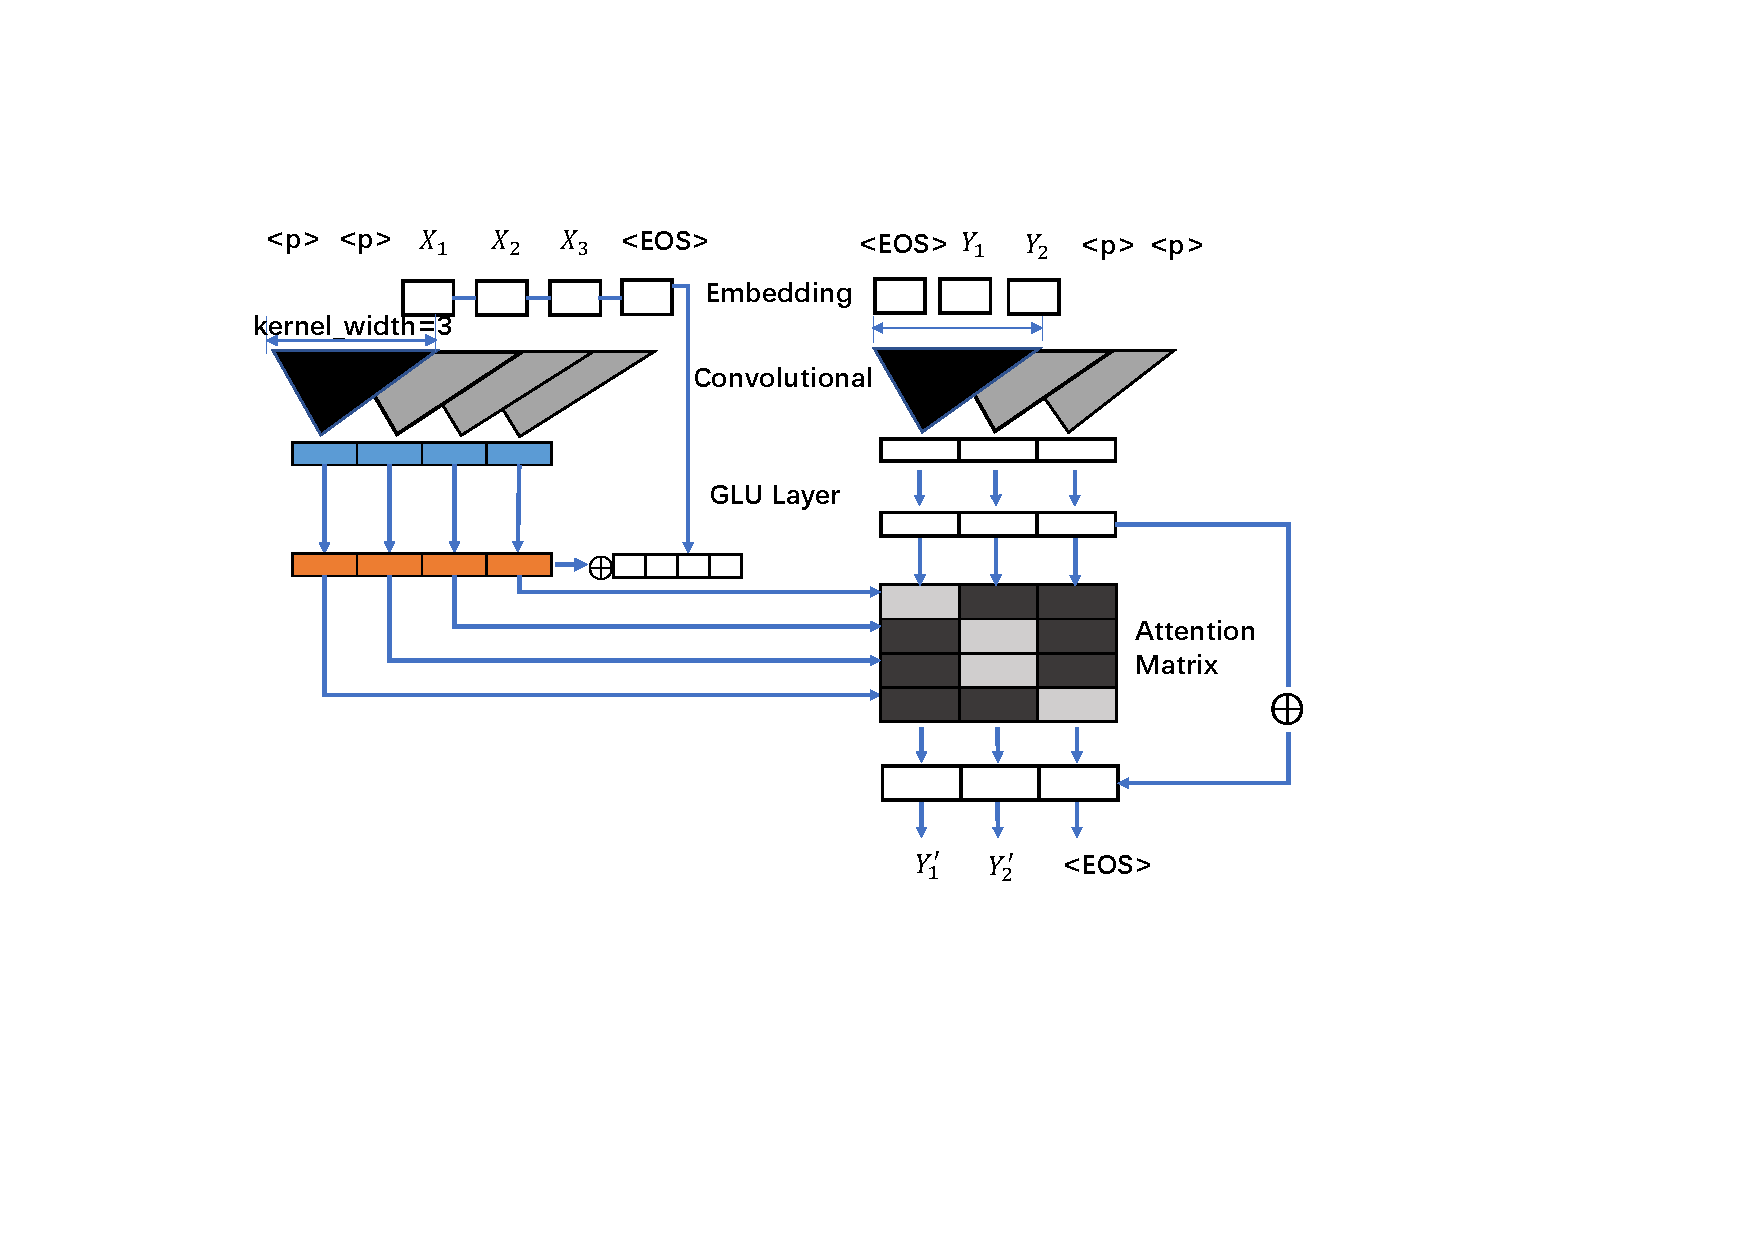
\includegraphics[width=1.0\columnwidth]{figure/cmodel}}
\caption{CNN seq2seq model} \label{fig:cnn}
\end{figure}

In the CNN seq2seq model, we obtain the input sequence
$\textbf{X}=(X_{1},...,X_{m})$ and output sequence $\textbf{Y}=(Y_{1},...,Y_{n})$
after combining word vectors with their absolute positions in the document.
%These sequences contain semantic and positional information. In this model,
%encoder and decoder are both based on multi-layers convolutional
%networks~\citep{CunBDHHHJ89}.
We use $\textbf{z}=(z^l_{1}, z^l_{2},..., z^l_{m})$ and
$\textbf{h}=(h^l_{1}, h^l_{2},..., h^l_{n})$
to denote the convolutional output of the encoder and decoder in $l$-th layer.
Each element of the output sequence generated by the decoder network
is fed back into the next layer of decoder network.
Next, we add GLU \cite{DauphinFAG17} and residual connections \cite{HeZRS16} 
in each layer:
%GLU is non-linearity and is used as a gate. This process is described
%as follows.
\begin{equation}
%h^l_{i} \!=\! GLU(W^l[h^{l-1}_{i-k/2},...,h^{l-1}_{i+k/2}]\!+\!b^l)\!+\!h^{l-1}_{i}
h^l_{i} \!=\! GLU(W^l[h^{l-1}_{s},...,h^{l-1}_{t}]\!+\!b^l)\!+\!h^{l-1}_{i}
\end{equation}
where $[h^{l-1}_{s},...,h^{l-1}_{t}]$ corresponds to the $h^l_{i}$ in the
convolutional layers. The choice of $s$ and $t$ is based on kernel width 
and the padding method used to match the output of convolutional layers to 
the input length.
We compute the probability distribution of generating the
next elements $y_{i+1}$ based
on the current state and transform the top decoder output $h^L_{i}$ via softmax:
\begin{equation}
p(y_{i+1}|y_{1},...,y_{i},\textbf{x})\!=\!softmax(W_{o}h^L_{i}\!+\!b_{o})
\end{equation}

In addition, a multi-step attention mechanism that connects the encoder and
decoder is used in each decoder layer. 
%It connects the encoder and decoder model after each GLU.
%To compute the attention, 
We define the decoder state $d^l_{i}$ for attention as following:
\begin{equation}
d^l_{i}\!=\!W^l_{d}h^l_{i}\!+\!b^l_{d}+Y_{i}
\end{equation}

The attention $c^l_{i}$ is a weighted sum of the encoder outputs.
The weights $a^l_{ij}$ are based on the decoder states.
%It can provide the distribution of next token given the input sequence.
\begin{align}
a^l_{ij} \!&=\! \frac {\exp(d^l_{i}\cdot z^u_{j})}{\sum^m_{t=1} \exp(d^l_{i}\cdot z^u_{t})} \\
c^l_{i}  \!&=\! \sum^m_{j=1} a^l_{ij}(z^u_{j}+X_{j})
\end{align}

At last, we add $c^l_{i}$ to the current decoder elements $h^l_{i}$,
which forms the final output or the
input of the next layer in the decoder.

\subsection{Modified Model with Length Control (LC)}
\label{sec:lc}
%To store and propagate the length requirement layer to layer,
%we add length embedding on the initializing the states of decoder.
We propose an approach which can control the summary length
in CNN seq2seq model.  The model can generate different summaries by
setting desired length. It has the ability to generate the EOS tag at the appropriate time
point in a natural manner. 
%\KZ{``Natural'' is the key word here. How do
%you measure natureness in your eval?}


To produce a summary of a given desired length,
we modify the basic model by feeding the desired length as
a parameter into the decoder of the CNN seq2seq model.
At training time, we use the true length of the gold summary as the
desired length. At test time, we can give any desired length $len$
to the model and obtain
a summary with length approximate to $len$.
The modified decoder is shown in \figref{fig:model}.

\begin{figure}[th]
\centering
\scalebox{1.0}{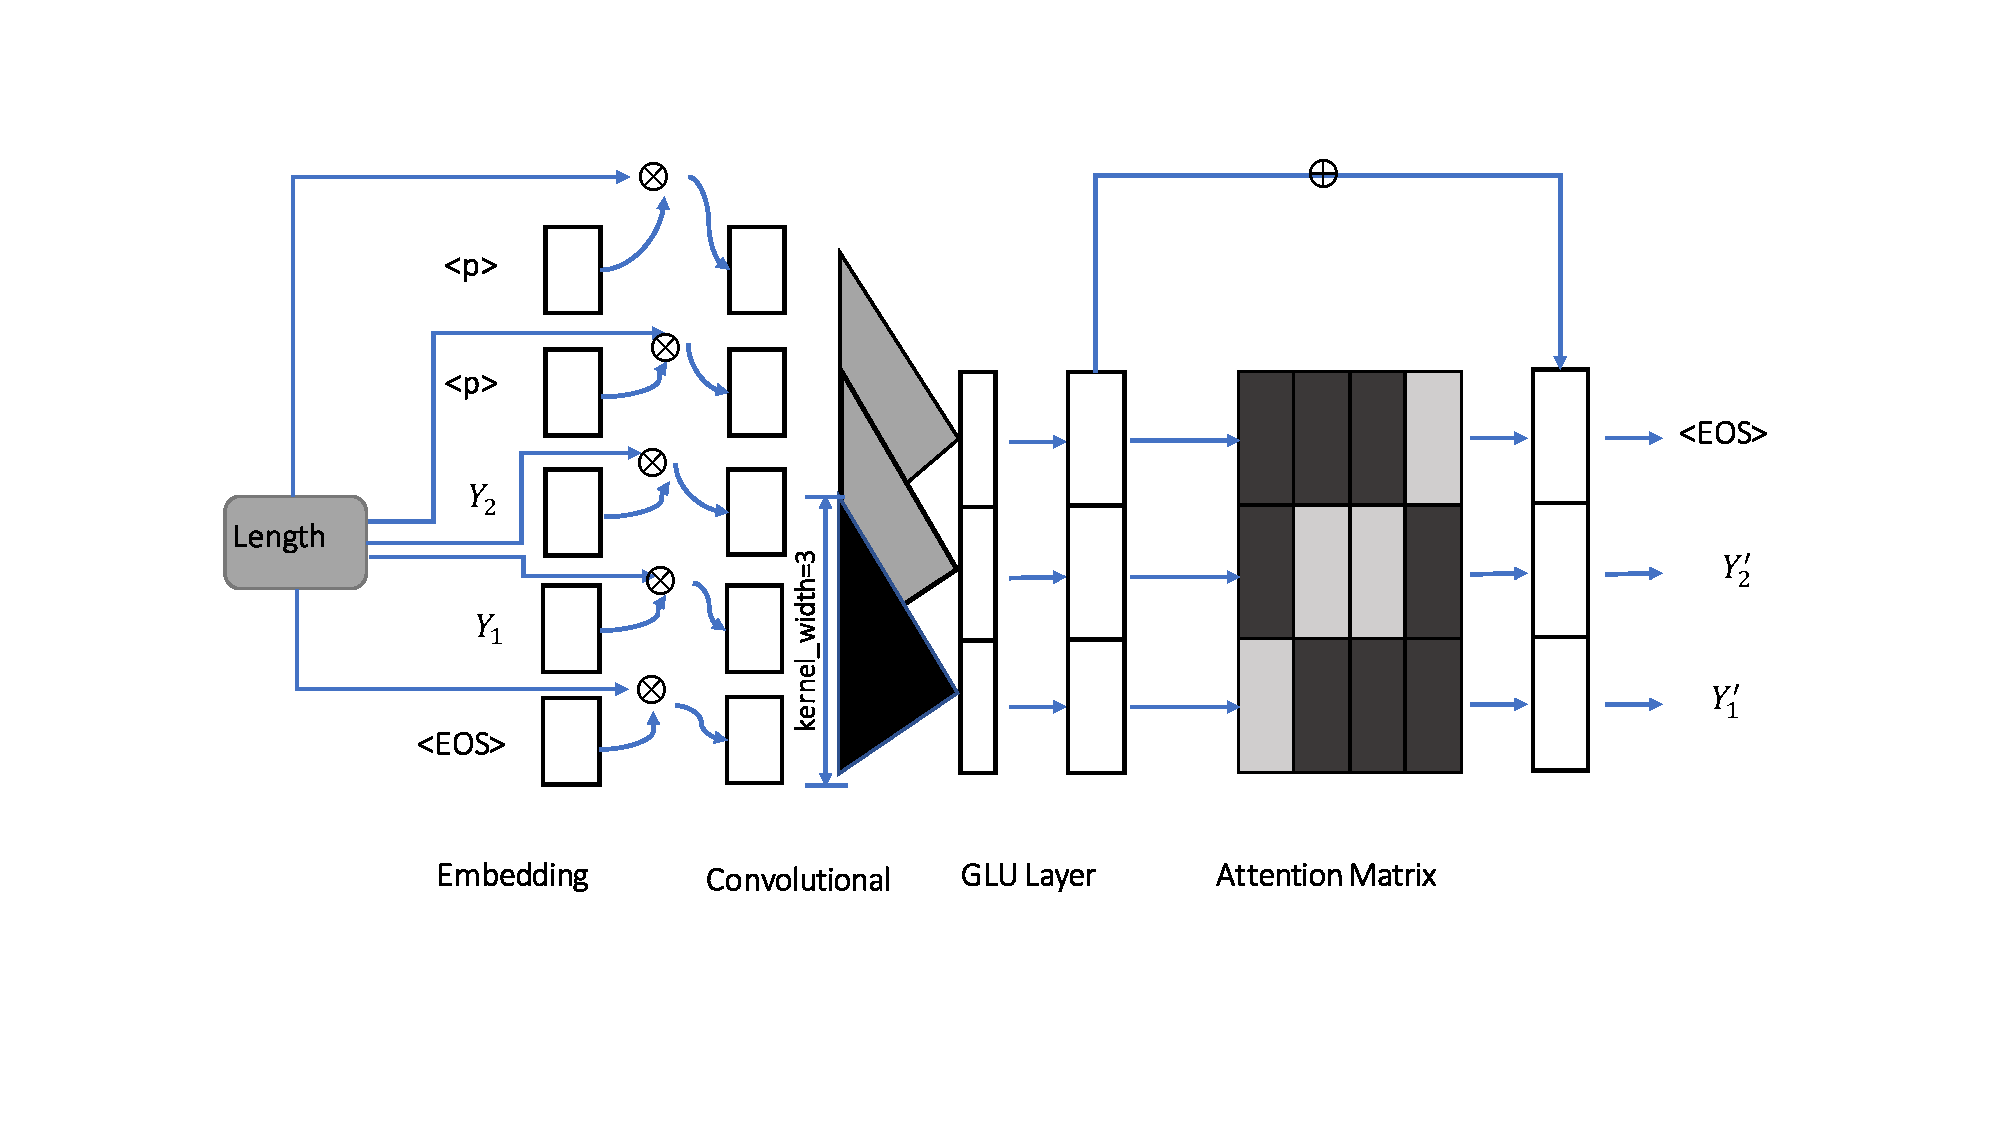
\includegraphics[width=1.0\columnwidth]{figure/length}}
\caption{Modified Decoder}
\label{fig:model}
\end{figure}


%In the other two models, we
%divided the training set into different buckets.
%Each bucket contain a kind of range that does not
%overlap with other buckets. We choose the ranges as \citep{abs-1711-05217},
%which ensures buckets contain roughly equal number of documents.
%Then, we add the exact range $target\_range$ which target summary
%belongs to into the decoder. At test time, we can give a desired range
%$(min, max)$ to the model and obtain
%a summary with length between $min$ and $max$.

%%\subsection{Length Control}
%
%At first, we will describe the length control method.
The CNN seq2seq model creates hierarchical
structure over the input sequence. It is capable of capturing the
correlation between elements over short distances at lower layers
and between elements over long distances at higher layers. 
The useful information among the elements is aggregated after GLU.
Therefore, we set the desired length as an input to the initial state of the decoder:
\begin{equation}
h^{1}_{i} \!=\! v(W^{1}[h^{0}_{s},...,h^{0}_{t}]\!+\!b^1)\!+\!h^{0}_{i}*len
\end{equation}
where $W$ is a trainable parameter, $len$ is the desired length, 
$v$ is GLU funciton and $h^{0}_{i}$ is the $i$-th element in the initial layer.

In the above function, we add length information at first 
layer in CNN model. GLU is like a gate. It can filter some information
from a particular unit in each layer. The information attenuation occurs in GLU
layer by layer. Different desired lengths have different degrees of information 
attenuation. Therefore the model is able to learn the probability of generating 
EOS with its own length information attenuation. 
This operation enables the model to produce a natural and complete summary 
for a given length constraint naturally. 
%Because it is possibale for GLU to learn 
%functions that, for example, filter some information
%from a particular unit in each layer.
%the multi-layer CNN network can propagate the length requirement from layer
%to layer.

%For controling summaries length of other methods and preventing summaries length 
%over 100~\footnote{The maximum length of summaries in CNN/DailyMail dataset is 94.}, 
%we use two methods.
%One is to truncate the generated summary when the length of output sequence is up to desired length $len$. It can limit
%the summary length less than $len$.
%The other is to ignore EOS token until the first $len$ tokens are generated and truncate the generated summary at $len$-th
%token. This can make sure that the summaries length exactly equals to the desired length.
%
\cut{%%%%%%%%%%%%%%%%%%%%%%%%%
\subsection{Length Range Control: Without Penalty (LRC)}

In this approach, we set the desired range as an input
to the initial state of the decoder (\figref{fig:model}). Different from the length, we redefine the representation of the desired
range. We use a 100-dimensional bit vector to represent the designed length
range, because the maximum length in the dataset is 100. The size of this
range vector can of course be adapted to the actual scenarios.
We set all bits that represent the desired range as 1 and all other bits 0.
For example, if the desired range is 10-30 words. Then the 10th bit through
30th bit of the vector are set to 1 while the rest set to 0.
%set $0$ to the other elements.
%For example, suppose that the max length is $10$ and the range is $(2,4]$, we will get
%$range = [0,0,0,1,1,0,0,0,0,0]$.

Then we use the softmax function to nomalized the original range vector
and get the normalized range vector $\textbf{r}$. We send the
normalized range vector to the initial layer.
\begin{equation}
h^{1}_{i} \!=\! v(W^{1}[h^{0}_{i-k/2},...,h^{0}_{i+k/2}]\!+\!b^1)\!+\!h^{0}_{i}*\textbf{r}\\
\end{equation}

This method can help us generate summaries in {\em any} length range
at test time while other existing methods can only generate summaries in
fixed, pre-defined ranges. For training, we should distribute the training
set into a set of buckets which denote different length range.
Each bucket is disjoint with other buckets and contains roughly
the equal number of documents \tabref{tab:datawithoutpenalty}.

\begin{table}[t!]
\small
\caption{The buckets for Fan et al.\shortcite{abs-1711-05217}. }
\label{tab:datawithoutpenalty}
\begin{center}
\begin{tabular}{|l|c|}
\hline \bf Buckets & \bf No. Examples\\ \hline
(0,33] & 29519 \\
(33,38] & 27679 \\
(38,42] & 28259 \\
(42,46] & 24722 \\
(46,50] & 24891 \\
(50,54] & 26990 \\
(54,59] & 30364 \\
(59,64] & 23641 \\
(64,72] & 25432 \\
(72,94] & 25697 \\
\hline
\end{tabular}
\end{center}
\end{table}

\subsection{Length Range Control: With Penalty (LRCP)}
The original negtive log-likelihood loss function(NLL) used in LRC
for each training pair is as follows:
\begin{equation}
NLL = -\log P(X|Y),
\end{equation}
where $P(X|Y)$ is the probability of a correct summary $X$ given the
source document $Y$.
With such a loss function, the model tends to produce summaries that
resembles the gold summary, because everything about the gold summary is
considered good, including the length of the gold summary. However, if
the distribution of the gold summary lengths is quite different from
the designed length at test time (e.g., most of the gold summary are from
80 words to 100 words, but the required summary length is 50), then
the above loss function and the LRC model will be insufficient.

Hence, in this new method called LRCP, while keeping the same length
range bucket settings as LRC, we redistribute the training data
such that half of the bucket contains documents with in
the designated length range and the other half contains documents
outside of this range.  This effectively creates a mix of
positive and negative examples in each bucket.
Meanwhile, we still ensure that each bucket contains roughly
equal number of documents. \tabref{tab:datawithpenalty}
shows the distribution of the buckets again.
\begin{table}[t!]
\small
\caption{ The buckets for LRCP. }
\label{tab:datawithpenalty}
\begin{center}
\begin{tabular}{|l|cc|}
\hline \bf Buckets & \bf Pos. Examples & \bf Neg. Examples\\ \hline
(0,33] & 14760 & 14751 \\
(33,38] & 13840 & 13833 \\
(38,42] & 14130 & 14121 \\
(42,46] & 12362 & 12357 \\
(46,50] & 12446 & 12438 \\
(50,54] & 13496 & 13491 \\
(54,59] & 15183 & 15174 \\
(59,64] & 11821 & 11817 \\
(64,72] & 12717 & 11869 \\
(72,94] & 12849 & 13739 \\
\hline
\end{tabular}
\end{center}
\end{table}

To enable length constraint,
we set $len$ to the true length of the summary in the training pair and let
$R = (R_{min}, R_{max}]$, where $R$ is the length range of the bucket to
which the training pair belongs.
Similar to LRC, $\textbf{r}$ is the corresponding nomalized range vecter.
We define a penalty factor $\mu$ as:
%If the real length of the summary in the range we allocate, $dist = 0$. If not, we compute the distance between the end of this Summary
%and the border of the pre-allocated range.
%\begin{equation}
%\mu \!=\! \left\{
%           \begin{array}{ll}
%           \alpha *\left|len-R_{min}\right| & {0 \!<\! len \leq R_{min}} \\
%           0 & {R_{min} \!<\! len \leq R_{max}} \\
%           \alpha *\left|len-R_{max}\right| & {len \!>\! R_{max}}
%           \end{array}
%           \right.
%\end{equation}
\begin{equation}
\mu =
\begin{cases}
\alpha *\left|len-R_{min}\right| & \text{, $0 \!<\!$ \textit{len} $\leq R_{min}$} \\
~~~~~~~~~~0 & \text{, $R_{min} \!<\!$ \textit{len} $ \leq R_{max}$} \\
\alpha *\left|len-R_{max}\right| & \text{, \textit{len} $\!>\! R_{max}$}
\end{cases}
\end{equation}

We do the same operation to the initial layer of model and use the
new NLL function:
\begin{equation}
NLL = -\log \frac{P(T|S)}{\exp(\mu)}
\end{equation}
}%%%%%%%%%%%%%
